\documentclass[11pt]{exam}
\usepackage{tikz}
\usepackage{soul}
\usetikzlibrary{positioning}
\usepackage[abs]{overpic}
\usepackage{pict2e}
\usepackage{listings}

\lstset{%
	language=Java,
	basicstyle=\footnotesize\ttfamily,
	numbers=left,
	numberstyle=\tiny,        
	xleftmargin=17pt,
        	xrightmargin=5pt,
	frame=single,
	breaklines=true,
	moredelim=**[is][\color{red}]{@}{@}
}

\lstdefinestyle{buggy}{
  language=Java,
  emptylines=1,
  breaklines=true,
  basicstyle=\ttfamily\color{black},
  moredelim=**[is][\color{red}]{@}{@},
}

\lstdefinestyle{correct}{
  language=Java,
  emptylines=1,
  breaklines=true,
  basicstyle=\ttfamily\color{black},
  moredelim=**[is][\color{blue}]{@}{@},
}

\makeatletter
\tikzset{
    block filldraw/.style={% only the fill and draw styles
        draw, fill=yellow!20},
    block rect/.style={% fill, draw + rectangle (without measurements)
        block filldraw, rectangle},
    block/.style={% fill, draw, rectangle + minimum measurements
        block rect, minimum height=0.8cm, minimum width=6em},
    from/.style args={#1 to #2}{% without transformations
        above right={0cm of #1},% needs positioning library
        /utils/exec=\pgfpointdiff
            {\tikz@scan@one@point\pgfutil@firstofone(#1)\relax}
            {\tikz@scan@one@point\pgfutil@firstofone(#2)\relax},
        minimum width/.expanded=\the\pgf@x,
        minimum height/.expanded=\the\pgf@y}}
\makeatother

\usepackage{titling}
\newcommand{\subtitle}[1]{%
  \posttitle{%
    \par\end{center}
    \begin{center}\large#1\end{center}
    \vskip0.5em}%
}
\usepackage{asymptote}
\usepackage{listings}
\usepackage[english]{babel}
\usepackage[pscoord]{eso-pic}% The zero point of the coordinate systemis the lower left corner of the page (the default).

\newcommand{\placetextbox}[3]{% \placetextbox{<horizontal pos>}{<vertical pos>}{<stuff>}
  \setbox0=\hbox{#3}% Put <stuff> in a box
  \AddToShipoutPictureFG*{% Add <stuff> to current page foreground
    \put(\LenToUnit{#1\paperwidth},\LenToUnit{#2\paperheight}){\vtop{{\null}\makebox[0pt][c]{#3}}}%
  }%
}%

\marksnotpoints

\begin{document}

\title{WCOM125/ COMP125 Week 1}
\subtitle{COMP115/ WCOM115 Revision}
\maketitle

\setcounter{page}{3}
\begin{questions}

\question What is the value of \texttt{result} when the following code is executed? Show your working using a logic table.

\begin{lstlisting}
int result = 3;
for(int i=1; i <= 20; i+=3) {
	if(i % 4 == 0) {
		result *= 2;
	}
	else {
		result--;
	}
}
\end{lstlisting}

\ifprintanswers \vskip 1cm \textbf{SOLUTION:} \vskip 1cm
\begin{tabular}{c|c|c|c|c}
  i & i $\le$ 20 & i \% 4 & i \% 4 == 0 & result\\
  \hline
  1 & true & 1 & false & 2\\
  4 & true & 0 & true & 4 \\
  7 & true & 3 & false & 3 \\
  10 & true & 2 & false & 2 \\
  13 & true & 1 & false & 1 \\
  16 & true & 0 & true & 2 \\
  19 & true & 3 & false & 1
\end{tabular}

Hence, result = 1
\newpage \else
\vskip 6cm 
\fi

\question
Write a piece of code that adds the first 100 positive integers (1 to 100) and stores the result in a variable \texttt{total}. You must use a loop in order to achieve this.

\ifprintanswers \vskip 1cm \textbf{SOLUTION:} \vskip 1cm
\begin{lstlisting}
int total = 0;
for(int i=1; i <= 100; i++) {
   total = total + i;
}
\end{lstlisting}
\newpage \else
\newpage
\fi

\question
What is the value of \texttt{result} when the following code is executed? Show your working using a logic table.

\begin{lstlisting}
int total = 0;
for(int i=1; i <= 10; i+=3) {
   for(int k=1; k <= i; k+=3) {
      result++;
   }
}
\end{lstlisting}

\ifprintanswers \vskip 1cm \textbf{SOLUTION:} \vskip 1cm
outer loop executes for i = 1,4,7,10
for i=1, inner loop executes for k=1
for i=4, inner loop executes for k=1,4
for i=7, inner loop executes for k=1,4,7
for i=10, inner loop executes for k=1,4,7,10

result increases 10 times, and becomes 10
\newpage \else
\newpage
\fi

\question
What is the value of \texttt{result} when the following code is executed? Show your working using a memory diagram.

\begin{lstlisting}
boolean foo(int n) {
	if(n > 5 && n < 10) {
		return true;
	}
	else {
		return false;
	}
}

void setup() {
	int a = 12;
	boolean result = foo(a);
}
\end{lstlisting}

\ifprintanswers \vskip 1cm \textbf{SOLUTION:} \vskip 1cm
result = false

the memory diagram should show two memory scopes (one for setup() and the other for foo(a). for the one in foo(a), the value of \texttt{a} should be copied into \texttt{n})
\newpage \else
	\vskip 4cm
\fi
\question
Define a function that when passed an integer, returns \texttt{true} if it's even (divisible by 2) and \texttt{false} otherwise.
 
\ifprintanswers \vskip 1cm \textbf{SOLUTION:} \vskip 1cm
\begin{lstlisting}
boolean isEven(int a) {
	if(a%2 == 0) {
		return true;
	}
	else {
		return false;
	}
}
\end{lstlisting}
\newpage \else
\newpage
\fi

\question
What is the value of \texttt{result} when the following code is executed? 

\begin{lstlisting}
int bar(int a, int b) {
	if(a > b)
		return a;
	else
		return b;
}

void setup() {
	int result = bar(bar(4,2), bar(3,6));
}
\end{lstlisting}

\ifprintanswers \vskip 1cm \textbf{SOLUTION:} \vskip 1cm
result = bar(4, 6) = 6
\newpage \else
	\vskip 3cm
\fi

\question
Define a function that when passed an integer (call it \texttt{num} in the scope of the function call), returns the sum of the first \texttt{num} positive integers. You may assume \texttt{num} $> 0$. For example, if \texttt{num = 4}, function should return 10 (1+2+3+4 = 10).

\ifprintanswers \vskip 1cm \textbf{SOLUTION:} \vskip 1cm
\begin{lstlisting}
int sum(int num) {
   int result = 0;
   for(int i=1; i <= num; i++) {
      result = result + i;
   }
   return result;
}
\end{lstlisting}
\newpage \else
\newpage
\fi

\question
What changes must you make to the function \texttt{sum} defined above if the assumption (\texttt{num} $> 0$) is no longer valid. What value do you think should be returned for \texttt{num} $\leq 0$

\ifprintanswers \vskip 1cm \textbf{SOLUTION:} \vskip 1cm
\begin{lstlisting}
int sum(int num) {
   if(num <= 0) {
      return 0;
   }
   
   int result = 0;
   for(int i=1; i <= num; i++) {
      result = result + i;
   }
   return result;
}
\end{lstlisting}
\newpage \else
\vskip 5cm
\fi

\question
Define a function that when passed two integers (call them \texttt{x, n} in the scope of the function call), returns the $x^n$ (\texttt{x * x * x ... n times}). You may assume \texttt{n} $> 0$. For example, if \texttt{x = 2, n = 4}, function should return 16 ($2^4 = 2*2*2*2 = 16$).

\ifprintanswers \vskip 1cm \textbf{SOLUTION:} \vskip 1cm
\begin{lstlisting}
int power(int x, int n) {
   int result = 1;
   for(int i=1; i <= n; i++) {
      result = result * x;
   }
   return result;
}
\end{lstlisting}
\newpage \else
\newpage
\fi

\question Create an array that holds 500 integers. Using a loop, populate the array, such that,

\begin{itemize}
	\item the first item is 5
	\item the second item is 7
	\item the third item is 9
	\item the fourth item is 11
	\item and so on
\end{itemize} 

\ifprintanswers
\begin{lstlisting}
int[] a = new int[500];
int val = 5;
for(int i=0; i < a.length; i++) {
	a[i] = val;
	val = val + 2;
}
\end{lstlisting}
\newpage
\else \vskip 8cm
\fi

\question Create an array that holds 100 real numbers. Using a loop, populate the array, such that,

\begin{itemize}
	\item the first item is 7.5
	\item the second item is 7.45
	\item the third item is 7.40
	\item the fourth item is 7.35
	\item and so on
\end{itemize} 

\ifprintanswers
\begin{lstlisting}
double[] a = new double[500];
double val = 7.5;
for(int i=0; i < a.length; i++) {
	a[i] = val;
	val = val - 0.05;
}
\end{lstlisting}
\newpage
\else \newpage
\fi

\question
Consider the following function definition,

\begin{lstlisting}
float square(float n) {
	return n*n;
}
\end{lstlisting}

Write one or two statements that sit inside the \texttt{setup()} function that calls the function \texttt{square} to compute $5^2$, and stores the returned value in a variable \texttt{result}. You must declare the variable \texttt{result} to an appropriate data type.
\ifprintanswers \vskip 1cm \textbf{SOLUTION:} \vskip 1cm
\begin{lstlisting}
float result = square(5);
\end{lstlisting}
\newpage \else
\vskip 3cm
\fi

\question Define a function \texttt{total} that when passed an integer array, returns the sum of all the items in the array. Return 0 if the array is \texttt{null}

\ifprintanswers \vskip 1cm \textbf{SOLUTION:} \vskip 1cm
\begin{lstlisting}[numbers=none, frame=single ,style=buggy]
int total(int[] a) {
	if(a == null)
		return 0;
	int result = 0;
	for(int i=0; i < a.length; i++) {
		result = result + a[i];
	}
	return result;
}	
\end{lstlisting}
\newpage \else
\newpage
\fi

\question What changes must you make to the function \texttt{total} defined above if you want to add \textbf{only the positive items}?

\ifprintanswers \vskip 1cm \textbf{SOLUTION:} \vskip 1cm
\begin{lstlisting}[numbers=none, frame=single ,style=buggy]
int totalEven(int[] a) {
	if(a == null)
		return 0;
	int result = 0;
	for(int i=0; i < a.length; i++) {
		@if(a[i] > 0) {@
			result = result + a[i];
		}
	}
	return result;
}	
\end{lstlisting}
\newpage \else
\vskip 6cm
\fi

\question What changes must you make to the function \texttt{total} defined above if you want to add \textbf{only the items in a specific range}. Say items that lie between:

\begin{itemize}
\item 1 and 6, or, 
\item 50 and 100
\end{itemize}

\ifprintanswers \vskip 1cm \textbf{SOLUTION:} \vskip 1cm
\begin{lstlisting}[numbers=none, frame=single ,style=buggy]
int totalInRange(int[] a, int low, int high) {
	if(a == null)
		return 0;
	int result = 0;
	for(int i=0; i < a.length; i++) {
		@if(a[i] >= low && a[i] <= high) {@
			result = result + a[i];
		}
	}
	return result;
}	
\end{lstlisting}
\newpage \else
\newpage
\fi

\question Define a function \texttt{highest} that when passed an integer array, returns the highest value in the array. Return 0 if the array is\texttt{null} or if the array is empty.

\ifprintanswers \vskip 1cm \textbf{SOLUTION:} \vskip 1cm
\begin{lstlisting}[numbers=none, frame=single ,style=buggy]
int highest(int[] a) {
	if(a == null)
		return 0;
	if(a.length == 0) //empty array
		return 0;
		
	int result = a[0]; //assume first item is the highest
	for(int i=1; i < a.length; i++) { //start from second item
		if(a[i] > result) {
			result = a[i];
		}
	}
	return result;
}	
\end{lstlisting}
\newpage \else
\vskip 10cm
\fi

\question What changes must you make to the function \texttt{highest} defined above if you want to return the \textbf{smallest item}.

\ifprintanswers \vskip 1cm \textbf{SOLUTION:} \vskip 1cm
\begin{lstlisting}[numbers=none, frame=single ,style=buggy]
int smallest(int[] a) {
	if(a == null)
		return 0;
	if(a.length == 0) //empty array
		return 0;
		
	int result = a[0]; //assume first item is the highest
	for(int i=1; i < a.length; i++) { //start from second item
		@if(a[i] < result) {@
			result = a[i];
		}
	}
	return result;
}	
\end{lstlisting}
\newpage \else
\newpage
\fi

\question Define a function \texttt{highestIndex} that when passed an integer array, returns the \textbf{index of} the highest value in the array. Return -1 if the array is\texttt{null} or if the array is empty.

\ifprintanswers \vskip 1cm \textbf{SOLUTION:} \vskip 1cm
\begin{lstlisting}[numbers=none, frame=single ,style=buggy]
int highestIndex(int[] a) {
	if(a == null)
		return 0;
	if(a.length == 0) //empty array
		return 0;
		
	int result = 0; //assume first item is the highest
	for(int i=1; i < a.length; i++) { //start from second item
		if(a[i] > a[result]) {
			result = i;
		}
	}
	return result;
}	
\end{lstlisting}
\newpage \else
\vskip 8cm
\fi

\question Which function is more powerful - \texttt{highest}, or \texttt{highestIndex}?
\ifprintanswers
\texttt{highestIndex} as we can get the item directly from index but not the index directly from the item.
\newpage
\else 
\vskip 2cm
\fi

\question What changes must you make to the function \texttt{highestIndex} defined above if you want to return the \textbf{index of the smallest item}.

\ifprintanswers \vskip 1cm \textbf{SOLUTION:} \vskip 1cm
\begin{lstlisting}[numbers=none, frame=single ,style=buggy]
int smallestIndex(int[] a) {
	if(a == null)
		return 0;
	if(a.length == 0) //empty array
		return 0;
		
	int result = 0; //assume first item is the smallest
	for(int i=1; i < a.length; i++) { //start from second item
		if(a[i] < a[result]) {
			result = i;
		}
	}
	return result;
}	
\end{lstlisting}
\newpage \else
\newpage
\fi

\question What changes must you make to the function \texttt{highest} defined above if you want to return the highest value \textbf{starting from a specific index}. For example, if \texttt{a = \{40, 80, 30, 50, 70, 20\}}, and the index starting at which we should look is 3 (note that a[3] is 50), the function returns 70
\ifprintanswers \vskip 1cm \textbf{SOLUTION:} \vskip 1cm
\begin{lstlisting}[numbers=none, frame=single ,style=buggy]
int highest(int[] a, int start) {
	if(a == null)
		return 0;
	if(start < 0 || start >= a.length) //invalid index
		return 0;
		
	int result = a[start]; //assume first item is the highest
	for(int i=start+1; i < a.length; i++) { //start from second item
		@if(a[i] > result) {@
			result = a[i];
		}
	}
	return result;
}	
\end{lstlisting}
\newpage \else
\vskip 7cm
\fi

\question What changes must you make to the function \texttt{highest} defined above if you want to return the \textbf{index of} the highest value \textbf{starting from a specific index}. For example, if \texttt{a = \{40, 80, 30, 50, 70, 20\}}, and the index starting at which we should look is 3 (note that a[3] is 50), the function returns 4 (item at index 4 is the highest starting at index 3).

\ifprintanswers \vskip 1cm \textbf{SOLUTION:} \vskip 1cm
\begin{lstlisting}[numbers=none, frame=single ,style=buggy]
int highestIndex(int[] a, int start) {
	if(a == null)
		return -1;
	if(start < 0 || start >= a.length) //invalid index
		return -1;
		
	int result = start; //assume first item is the highest
	for(int i=start+1; i < a.length; i++) { //start from second item
		@if(a[i] > a[result]) {@
			result = i;
		}
	}
	return result;
}	
\end{lstlisting}
\newpage \else
\newpage
\fi


\question Define a function \texttt{identical} that when passed two integer arrays, returns \texttt{true} if they are identical to each other, \texttt{false} otherwise (or if either of the arrays is \texttt{null}).

\ifprintanswers \vskip 1cm \textbf{SOLUTION:} \vskip 1cm
\begin{lstlisting}[numbers=none, frame=single ,style=buggy]
boolean identical(int[] a, int[] b) {
	if(a == null || b == null)
		return false;
	if(a.length != b.length)
		return false;
	for(int i=0; i < a.length; i++) {
		if(a[i] != b[i]) {
			return false;
		}
	}
	return true;
}	
\end{lstlisting}
\newpage \else
\vskip 10cm
\fi

\question \textbf{(advanced)}
Define a function \texttt{withoutFirstDigit} that when passed an integer $n$, returns the number without the first digit. You may assume that $m$ is more than 0. For example, if $m=7129$, function returns 129.

\ifprintanswers \vskip 1cm \textbf{SOLUTION:} \vskip 1cm
\begin{lstlisting}
int withoutFirstDigit(int m) {
  int result=  0;
  int power = 1;
  while (m != 0) {
    if (m > 9) {
      result = m%10 * power + result;
    }
    power*=10;
    m/=10;
  }
  return result;
}
\end{lstlisting}
OR
\begin{lstlisting}
int withoutFirstDigit(int m) {
	if(m == 0)
		return 0;
	m = Math.abs(m);
	String s = m+"";
	int result = Integer.parseInt(s.substring(1));
	return result;
}
\end{lstlisting}
\newpage \else
\newpage
\fi

\question Draw the memory diagram that captures the transactions when the following code executes.

\begin{lstlisting}
int[] a = {1, 7, 2};
int[] b = a;
int[] c = new int[a.length];
for(int i=0; i < a.length; i++) {
	c[i] = a[i];
}
\end{lstlisting}

\ifprintanswers \vskip 1cm \textbf{SOLUTION:} \vskip 1cm
%\begin{tikzpicture}[scale=.3]
%	\draw (0, 0) rectangle (8, 30);
%	\foreach \y in {2, 4, ..., 28} {
%		\draw (0, \y) -- (8, \y);
%	}
%	\node (a) at (2, 29) {$a$};
%	\node (b) at (2, 17) {$b$};
%	\node (a0) at (3, 25) {[0] = 1};
%	\node (a1) at (3, 23) {[1] = 7};
%	\node (a2) at (3, 21) {[2] = 2};
%	\node (c) at (2, 13) {$c$};
%	\node (c0) at (3, 7) {[0] = 1};
%	\node (c1) at (3, 5) {[1] = 7};
%	\node (c2) at (3, 3) {[2] = 2};
%
%\draw[->,line width=2pt] (0, 29.5) .. controls (-5, 27) .. (0, 25.5);
%\draw[->,line width=2pt] (0, 17.5) .. controls (-5, 23) .. (0, 25.5);
%\draw[->,line width=2pt] (0, 13.5) .. controls (-5, 10) .. (0, 7.5);
%\end{tikzpicture}

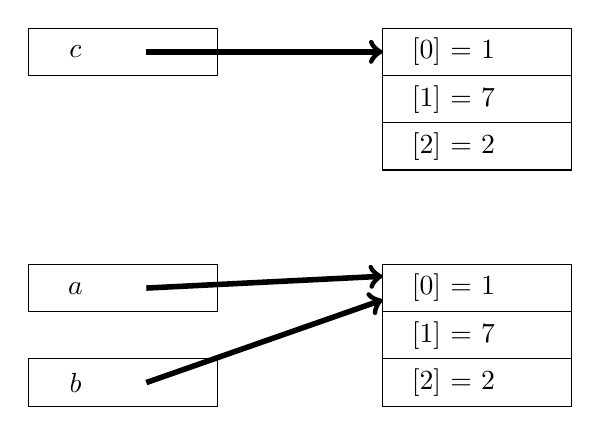
\begin{tikzpicture}[scale=.3]
	\draw (0, 16) rectangle (8, 18);
	\node (a) at (2, 17) {$a$};

	\draw (15, 12) rectangle (23, 18);
	\foreach \y in {14, 16} {
		\draw (15, \y) -- (23, \y);
	}

	\node (a0) at (18, 17) {[0] = 1};
	\node (a1) at (18, 15) {[1] = 7};
	\node (a2) at (18, 13) {[2] = 2};
	
	\draw[->,line width=2pt] (5, 17) .. controls (10, 17.25) .. (15, 17.5);

	\draw (0, 12) rectangle (8, 14);
	\node (b) at (2, 13) {$b$};

	\draw[->,line width=2pt] (5, 13) .. controls (10, 14.75) .. (15, 16.5);


	\draw (0, 26) rectangle (8, 28);
	\node (c) at (2, 27) {$c$};

	\draw (15, 22) rectangle (23, 28);
	\foreach \y in {24, 26} {
		\draw (15, \y) -- (23, \y);
	}

	\node (c0) at (18, 27) {[0] = 1};
	\node (c1) at (18, 25) {[1] = 7};
	\node (c2) at (18, 23) {[2] = 2};
	
	\draw[->,line width=2pt] (5, 27) .. controls (10, 27) .. (15, 27);


\end{tikzpicture}


\else
\newpage
\fi
\end{questions}
\end{document}
